\chapter{Estado del arte}
La selección de características es un problema cuya popularidad ha ido en aumento con el paso de los años. No es algo casual, pues la cantidad de datos recogidos para tareas de aprendizaje automático y áreas derivadas, como el aprendizaje profundo, ha ido en aumento de manera casi exponencial.

\begin{figure}[H]
    \begin{center}
        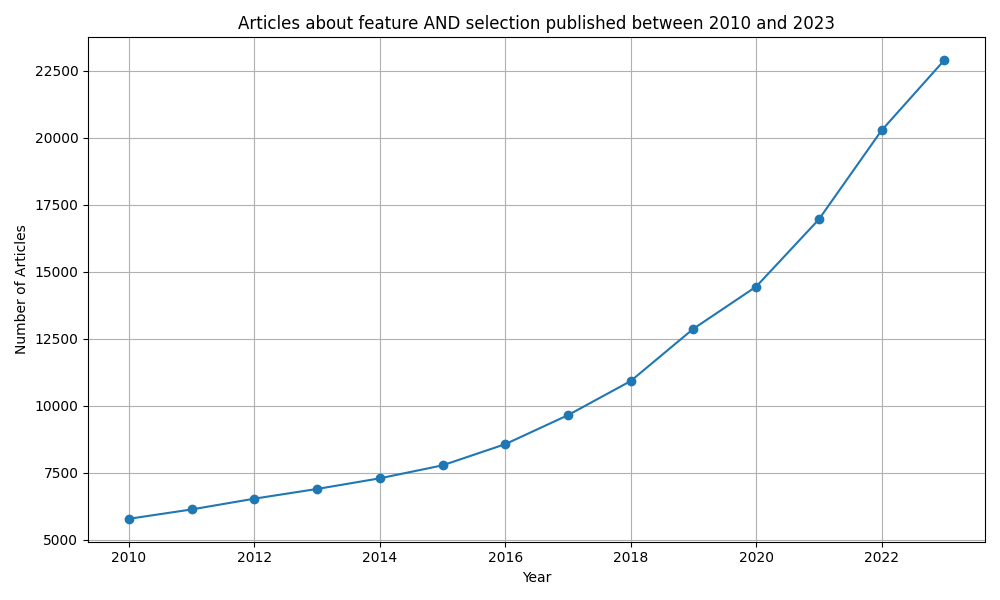
\includegraphics[width=1\textwidth]{imagenes/scopus_chart.png}
    \end{center}
    \caption[Popularidad de feature selection sobre los años]{En esta figura se muestra el número de artículos publicados relacionados con la selección de características. Se ha usado el buscador Scopus.}
    \label{fig:pop_fs}
\end{figure}

También se puede observar una tendencia  prácticamente igual en la popularidad sobre los años del problema de selección de características, pero abordado con técnicas metaheurísticas.

\begin{figure}[H]
    \begin{center}
        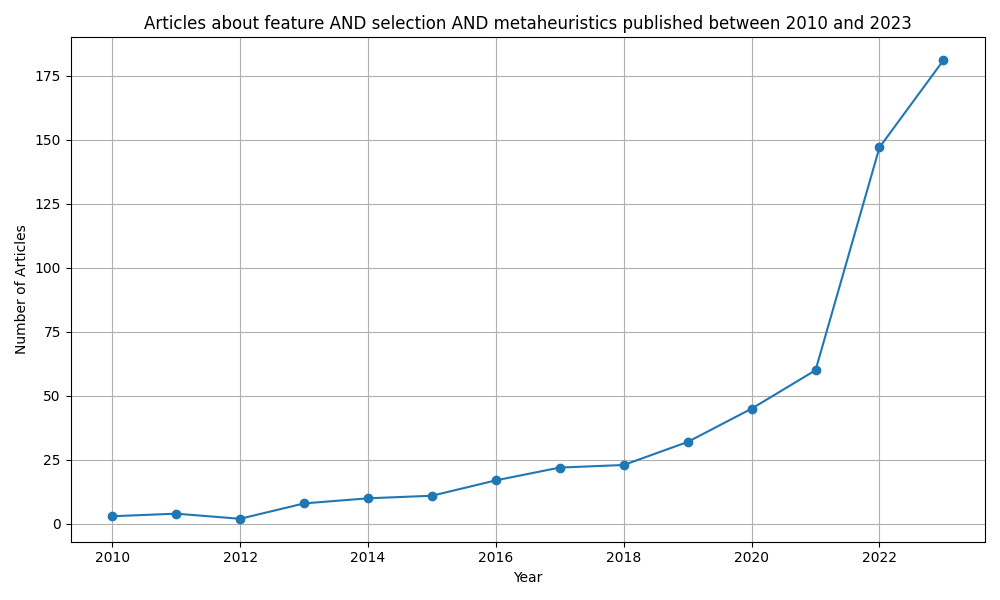
\includegraphics[width=1\textwidth]{imagenes/scopus_chart2.png}
    \end{center}
    \caption[Popularidad de feature selection + metaheuristics sobre los años]{De igual forma que en la figura \ref{fig:pop_fs} las mateheuristicas han ido muy ligadas a la resolución de este problema. Se ha usado el buscador Scopus.}
\end{figure}

Y es que las metaheurísticas son algoritmos muy convenientes en la resolución de este tipo de problemas. Algoritmos analíticos no son válidos cuando el conjunto de datos tiene un número de características muy elevado debido a una cantidad de combinaciones simplemente inabordable en términos computacionales. Debido a ello, se suelen utilizar algoritmos más rápidos cuya solución no es óptima globalmente hablando, pero si suficientemente buena.\\[6pt]
Muchos algoritmos metaheurísticos han sido propuestos a lo largo de los años. Se han escogido los más destacables en cuanto a resultados y más mencionados entre todos ellos, dando una selección de algoritmos metaheurísticos modernos de, en principio, muy alta calidad. No solo son seleccionados algoritos modernos, sino que también se han escogido una serie de algoritmos más ``clásicos'', pero cuya aplicación es más extendida y con resultados que, de forma empírica, han demostrado ser más que buenos a lo largo de décadas de uso.

\begin{table}[H]
    \parbox{.45\linewidth}{
        \centering
        \begin{tabular}{l}
            \hline
            Algoritmos \\ \hline
            GWO        \\
            FA         \\
            GOA        \\
            WOA        \\
            DA         \\
            CS         \\
            BA         \\
            \hline
        \end{tabular}
        \caption{Algoritmos modernos}
    }
    \hfill
    \parbox{.45\linewidth}{
        \centering
        \begin{tabular}{l}
            \hline
            Algoritmos \\ \hline
            PSO        \\
            GA         \\
            ACO        \\
            DE         \\
            ABCO       \\
            \hline
        \end{tabular}
        \caption{Algoritmos clásicos}
    }
\end{table}

\section{Algoritmos genéticos}
\subsection{Introducción}
Los algoritmos genéticos están inspirados en la selección natural y se utilizan tanto en problemas de optimización con restricciones como sin ellas. Es una metaheurística que modifica una población de soluciones individuales de manera repetida, seleccionando soluciones ``padre'' que dan lugar a la siguiente generación de soluciones en la siguiente iteración del algoritmo. En su forma más básica, un algoritmo genético opera sobre una población de soluciones potenciales a un problema dado. Cada solución potencial, a menudo llamada individuo o cromosoma, está representada como una cadena de símbolos, que puede ser binaria, numérica o simbólica~\cite{10.5555/522098}.

\subsection{Representación y Proceso}
Las soluciones o \textbf{fenotipos} están compuestas por una serie de propiedades, características, cromosomas o \textbf{genotipos}, que pueden ser mutados y alterados. La representación más común es la binaria, pero otras codificaciones son posibles.

El proceso típico incluye~\cite{mathew2012genetic}:
\begin{itemize}
    \item Inicialización aleatoria de la población.
    \item Evaluación del \textit{fitness} de cada individuo.
    \item Selección de padres basada en el \textit{fitness}.
    \item Creación de una nueva generación mediante cruces y mutaciones.
    \item Elitismo: selección de los mejores individuos~\cite{mirjalili2019genetic}.
\end{itemize}

\begin{figure}[H]
    \begin{center}
        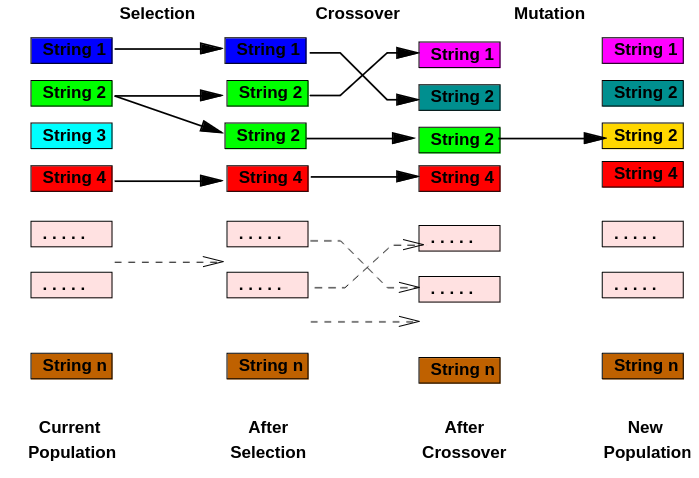
\includegraphics[width=0.6\textwidth]{imagenes/ga-working-principle.png}
    \end{center}
    \caption[Funcionamiento de un algoritmo genético]{Figura obtenida de \cite{mathew2012genetic}}
\end{figure}


El algoritmo termina cuando se alcanza cierta tolerancia de error o número máximo de iteraciones.

\subsubsection{Selección}
La selección se puede llevar a cabo con varios métodos, uno de los más utilizados en selección por torneo.\\[6pt]
En la selección por torneo, los individuos compiten entre sí en grupos pequeños. Cada grupo (torneo) tiene varios competidores (individuos). El competidor con la mejor aptitud (\textbf{fitness}) dentro del grupo gana y se selecciona para reproducirse. Este proceso se repite hasta que se completa el \textit{pool} de apareamiento con los ganadores de los torneos~\cite{miller_genetic_nodate}.

\subsubsection{Cruce}
Existen múltiples tipos de crossover o cruces. Se describen los dos usados en este proyecto (uno para la versión binaria del algoritmo y otra para la real):
\begin{itemize}
    \item \textbf{One-point crossover}: Se elige al azar un punto en los cromosomas de ambos progenitores y se designa como "punto de cruce". Los bits a la derecha de ese punto se intercambian entre los dos cromosomas parentales. El resultado son dos descendientes, cada uno con información genética de ambos progenitores~\cite{DAGDIA2020283}.
          \begin{figure}[H]
              \begin{center}
                  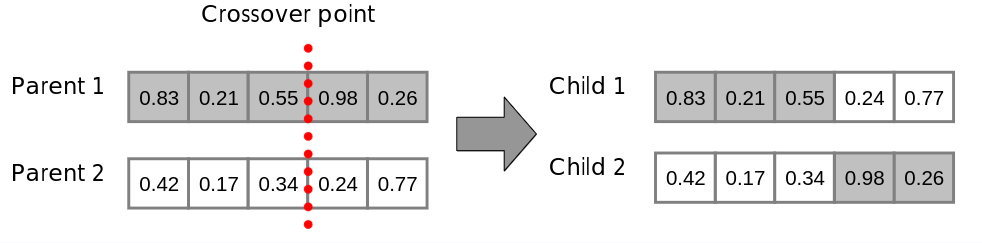
\includegraphics[width=0.6\textwidth]{imagenes/one-point-crossover.png}
              \end{center}
              \caption[One point crossover]{One-point crossover~\cite{purduelecture}}
          \end{figure}
    \item \textbf{Blend crossover}: Dado dos números reales para cada uno de los genes de los padres al hijo se le asignará un número aleatorio entre ese rango de gen para cada gen que conforme al vector cromosómico~\cite{purduelecture}.
          \begin{figure}[H]
              \begin{center}
                  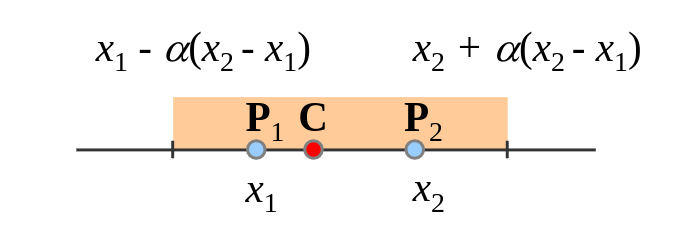
\includegraphics[width=0.6\textwidth]{imagenes/blend-crossover.png}
              \end{center}
              \caption[Blend crossover]{Blend crossover~\cite{purduelecture}}
          \end{figure}
\end{itemize}

\subsubsection{Mutación}
Su propósito es mantener la diversidad genética de los cromosomas de una población de un algoritmo evolutivo.
El operador más básico y clásico consiste en cambiar un bit arbitrario de un genotipo o solución de un algoritmo genético binario a su estado inverso dada una probabilidad de mutación~\cite{mirjalili2019genetic}.

\subsubsection{Elitismo}
El elitismo garantiza que las soluciones de alta calidad sobrevivan en las generaciones futuras, ayudando en la explotación del espacio de búsqueda. La cantidad de individuos élite seleccionados debe ser elegida con precisión~\cite{mirjalili2019genetic}.

\section{Algoritmos de colonias de hormigas}
\subsection{Introducción}
El algoritmo de colonia de hormigas o \textbf{ACO} es una técnica probabilística que trata de resolver problemas computacionales que pueden ser reducidos a la búsqueda de caminos óptimos a través de grafos. Se basa en el comportamiento de las hormigas reales y su comunicación vía feromonas. Las hormigas vagan por el mundo en búsqueda de comida de forma aleatoria. Cuando estas encuentran comida, dejan trazas de feromonas en su camino, de esta forma, si otras hormigas encuentran ese rastro, se hace más probable que recorran ese camino y dejen de vagar de forma aleatoria. Sin embargo, las trazas de feromonas se evaporan con el tiempo, perdiendo su fuerza de atracción sobre otras hormigas. De esta forma, si el camino es muy largo, la hormiga tardará mucho en recorrerlo y la traza de feromonas tendrá más tiempo a evaporarse. De manera análoga, a más corto es el camino, más rápido se recorre y más densidad de feromonas acumula~\cite{kashef_advanced_2015}.

\subsection*{Representación}
Para poder adaptar el algoritmo ACO a un problema es necesario reducir ese problema a la búsqueda del camino más corto dentro de un grafo ponderado.

\subsection*{ACO Feature Selection}
Cada característica del problema original se representa como un nodo $n$. Los caminos que conectan a los nodos ($e$) representan la elección del subconjunto de características. El camino deberá ser lo más corto posible maximizando a su vez el \textbf{accuracy}~\cite{kashef_advanced_2015}.

\subsubsection*{Regla de transición probabilística}
\[
    P_{ij}^k(t)=\begin{cases} \frac{\tau_{ij}^{\alpha}\eta_{ij}^{\beta}}{\sum_l\tau_{il}^{\alpha}\eta_{il}^{\beta}} & \text{Si $l$ y $k$ son nodos admisibles} \\ 0 & \text{De lo contrario} \end{cases}
\]
Donde:
\begin{itemize}
    \item $P_{ij}^k(t)$ denota la probabilidad de transición de un nodo de $i$ a $j$ en la $k$-hormiga (agente) en el instante de tiempo $t$.
    \item $\tau_{ij}$ es la cantidad de traza de feromona en la arista $(i,j)$ en el momento $t$. $\eta_{ij}$ es la heurística de deseabilidad o visibilidad de la arista.
    \item $\beta$ y $\alpha$ son dos parámetros que controlan la importancia relativa del valor de la feromona vs la información de la heurística.
\end{itemize}

Después de que todas las hormigas hayan terminado su camino, la evaporación de feromonas comienza. El contenido de feromonas del camino $(i,j)$ en el instante $t+1$ es:
\[
    \tau_{ij}(\text{new})=(1-p)\tau_{ij}(t)+\sum_{k=1}^m\Delta\tau_{ij}^k(t)+\Delta\tau_{ij}^g(t)
\]
Donde:
\begin{itemize}
    \item $\Delta\tau_{ij}^k=\begin{cases}\frac{Q}{F^k}&\hspace{6mm}\text{Si la hormiga k pasa por la arista (i,j) en }T^k\\0 &\hspace{6mm}\text{De lo contrario}\end{cases}$
    \item $p\in (0,1]$ es el ritmo de evaporación.
    \item $m$ es el número de hormigas.
    \item $\Delta\tau_{ij}^k$ y $\Delta\tau_{ij}^g$ son respectivamente, la cantidad de feromonas colocadas en la arista $(i,j)$ por la hormiga $k$ y la cantidad de feromonas depositadas por la mejor hormiga $g$ en el instante $t$ sobre la arista $(i,j)$.
    \item $Q$ es una constante y $F^k$ es el valor de coste de la solución encontrada por la hormiga $k$ en el tour $T^k$, es decir, $F^k$ es el \textit{fitness} de la hormiga $k$.
\end{itemize}
Se utiliza el sistema \textit{max-min}, solo la mejor hormiga puede depositar feromona.

\subsubsection*{bACO}
Este algoritmo usaba la estrategia \textit{max-min}, permitiendo solo a la mejor hormiga depositar feromona y limitando el valor de esta entre un valor mínimo y uno máximo~\cite{kashef_advanced_2015}.

\section{Optimización por enjambre de partículas}